\documentclass[border=4pt]{standalone}
% Preámbulo común de las figuras. Cada figura es un documento standalone
% que se compila a SVG con scripts/build_figures.sh
\usepackage[utf8]{inputenc}
\usepackage{amsmath}
\usepackage{tikz}
\usepackage[american, siunitx]{circuitikz}
\usetikzlibrary{arrows.meta,calc,decorations.pathmorphing,patterns}
\tikzset{
  >={Stealth[length=2.2mm]},
  eje/.style={->, thin},
  hilo/.style={thick},
}
% Paleta común: tonos medios legibles sobre fondo claro
\definecolor{azul}{RGB}{31,94,168}
\definecolor{rojo}{RGB}{192,57,43}
\definecolor{verde}{RGB}{39,128,73}
\definecolor{naranja}{RGB}{211,120,30}
\definecolor{morado}{RGB}{125,60,152}

\begin{document}
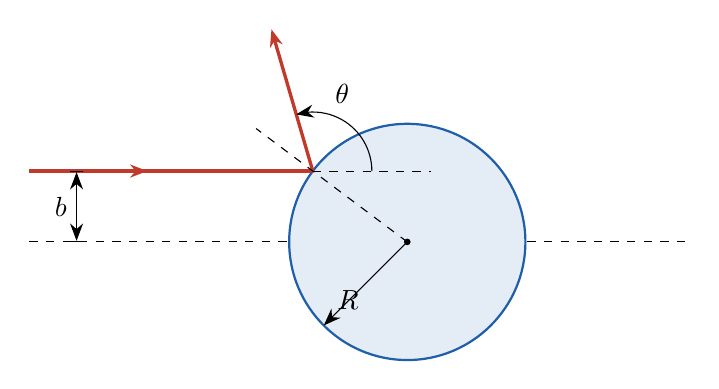
\begin{tikzpicture}[scale=1.5]
  % R = 1, b = 0.6: incidencia a 36.87 grados de la normal, desviacion de 106.26 grados
  \draw[dashed, thin] (-3.2,0) -- (2.4,0);
  \filldraw[draw=azul, fill=azul!12, thick] (0,0) circle (1);
  \fill (0,0) circle (0.8pt);
  \draw[->] (0,0) -- node[below left=-1pt]{$R$} (225:1);
  \draw[very thick, rojo] (-3.2,0.6) -- (-0.8,0.6);
  \draw[->, very thick, rojo] (-3.2,0.6) -- (-2.2,0.6);
  \draw[very thick, rojo, ->] (-0.8,0.6) -- ++(106.26:1.25);
  \draw[dashed, thin] (0,0) -- ++(143.13:1.6);
  \draw[dashed, thin] (-0.8,0.6) -- ++(0:1.0);
  \draw[->] (-0.3,0.6) arc (0:106.26:0.5);
  \node at (-0.55,1.25) {$\theta$};
  \draw[|<->|] (-2.8,0) -- node[left]{$b$} (-2.8,0.6);
\end{tikzpicture}
\end{document}
